\documentclass[12pt]{ustcreport}

\school{计算机}			%系
\year{21}			%级
\name{常文正}		%姓名
\date{2022-3-31}			%日期 
\No{PB21111706}		%No.
\title{液体表面张力系数测定}

\usepackage{multirow}
\usepackage{float}
\usepackage{amsmath}
\usepackage{fontspec}
\setmainfont{Times New Roman}
\usepackage{ctex}
\usepackage{lipsum}

\linespread{1}

\begin{document}
\section{实验目的}
液体具有尽量缩小其表面的趋势,好象液体表面是一张拉紧了的橡皮膜一样。把这种沿
着表面的、收缩液面的力称为表面张力。表面张力的存在能说明物质处于液态时所特有的许
多现象,比如泡沫的形成、润湿和毛细现象等等。
测定液体表面张力的方法很多,常用的有焦利氏秤法(拉脱法)、毛细管法、平板法、
滴重法、最大泡压法等。
本实验采用焦利氏秤法(拉脱法)。该方法的特点是,用秤量仪器直接测量液体的表面
张力,测量方法直观,概念清楚。
\section{实验原理}
液体表面层(其厚度等于分子的作用半径)内的分子所处的环境跟液体内部的分子是不
同的。
表面层内的分子合力垂直于液面并指向液体内部, 所以分子有从液面挤入液体内部的倾
向,并使液体表面自然收缩
想象在液面上划一条直线,表面张力就表现为直
线两旁的液膜以一定的拉力相互作用。拉力 F 存在
于表面层,方向恒与直线垂直,大小与直线的长度
l 成正比,
即
\begin{equation*}
    F = \sigma l
\end{equation*}
式中$\sigma $称为表面张力系数,它的大小与液体的
成分、纯度、浓度以及温度有关。
\section{实验装置}
焦利秤的构造如图所示,它实际上是一种用于测
微小力的精细弹簧秤。一般的弹簧秤都是弹簧秤上端
固定,在下端加负载后向下伸长,而焦利秤与之相反,
它是控制弹簧下端的位置保持一定,加负载后向上拉
动弹簧确定伸长值。
\begin{figure}[H]
    \centering
    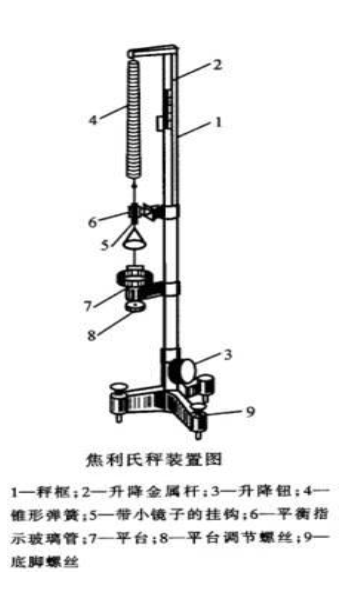
\includegraphics[width = 0.3\linewidth]{BMZLSYZZ.png}
    \label{mylabel1}
\end{figure}
\section{原始数据}
\begin{table}[H]
    \centering
    \begin{tabular}{|c|c|c|c|c|c|c|c|c|c|c|}
    \hline
    质量m/g  & 0.5  & 1.0  & 1.5  & 2.0  & 2.5  & 3.0  & 3.5  & 4.0  & 4.5  & 5.0  \\ \hline
    距离x/cm & 3.91 & 4.39 & 4.82 & 5.28 & 5.75 & 6.23 & 6.68 & 7.16 & 7.63 & 8.08 \\ \hline
    \end{tabular}
\end{table}
\begin{table}[H]
    \centering
    \begin{tabular}{|lll|lll|}
    \hline
    \multicolumn{3}{|l|}{距离s/cm}                                  & \multicolumn{3}{l|}{直径d/cm}                                  \\ \hline
    \multicolumn{1}{|l|}{4.20} & \multicolumn{1}{l|}{4.15} & 4.17 & \multicolumn{1}{l|}{3.85} & \multicolumn{1}{l|}{3.63} & 3.75 \\ \hline
    \end{tabular}
\end{table}
\begin{table}[H]
    \centering
    \begin{tabular}{|c|c|c|ccccc|}
    \hline
    测量液体 & 测量组件 & 初始距离$l_0$/cm & \multicolumn{5}{c|}{破裂时的距离l/cm}                                                                                      \\ \hline
    自来水  & 金属圈  & 8.07        & \multicolumn{1}{c|}{9.34} & \multicolumn{1}{c|}{9.44} & \multicolumn{1}{c|}{9.40} & \multicolumn{1}{c|}{9.41} & 9.42 \\ \hline
    洗洁精  & 金属丝  & 8.00        & \multicolumn{1}{c|}{8.21} & \multicolumn{1}{c|}{8.09} & \multicolumn{1}{c|}{8.20} & \multicolumn{1}{c|}{8.21} & 8.20 \\ \hline
    酒精   & 金属丝  & 8.00        & \multicolumn{1}{c|}{8.20} & \multicolumn{1}{c|}{8.17} & \multicolumn{1}{c|}{8.17} & \multicolumn{1}{c|}{8.19} & 8.16 \\ \hline
    \end{tabular}
\end{table}
% Please add the following required packages to your document preamble:
% \usepackage{multirow}
\begin{table}[H]
    \centering
    \begin{tabular}{|c|c|c|c|c|c|c|}
    \hline
    测量液体                      & 测量组件                 & 初始距离$l_0$/cm           & 浓度(体积比)                     & 1/100 & 1/10000 & 1/1000000 \\ \hline
    \multirow{2}{*}{不同浓度的洗洁精} & \multirow{2}{*}{金属丝} & \multirow{2}{*}{8.00} & \multirow{2}{*}{破裂时的距离l/cm} & 8.20  & 8.25    & 8.45      \\ \cline{5-7} 
                              &                      &                       &                             & 8.21  & 8.24    & 8.43      \\ \hline
    \end{tabular}
\end{table}
\section{数据处理}
\begin{enumerate}
    \item 最小二乘法/作图法求弹簧劲度系数:\\
    由公式:
    \begin{equation*}
        F = mg = k(x-x_0)
    \end{equation*}
    可得:
    \begin{equation*}
        x = \frac{g}{k}m + x_0
    \end{equation*}
    将原始数据换算成国际单位计算:
    \begin{equation*}
        \overline{m} = \frac{\sum_{i = 1}^10 m_i}{10} = 2.75*10^{-3}\mathrm{kg}
    \end{equation*}
    \begin{equation*}
        \overline{x} = \frac{\sum_{i = 1}^10 x_i}{10} = 0.0599\mathrm{m}
    \end{equation*}
    利用最小二乘法y = bx + a可得:
    \begin{equation*}
        b = \frac{g}{k} = \frac{\sum_{i=1}^{10}m_ix_i-10\overline{x}\overline{m}}{\sum_{i=1}^{10}m_i^2-10\overline{m}^2} = 9.2836364 \mathrm{m}/\mathrm{kg}
    \end{equation*}
    进而可计算出k为
    \begin{equation*}
        k = \frac{g}{b} = 1.05 \mathrm{N}/\mathrm{m} 
    \end{equation*}
    将统计输入origin作图可得:
    \begin{figure}[H]
        \centering
        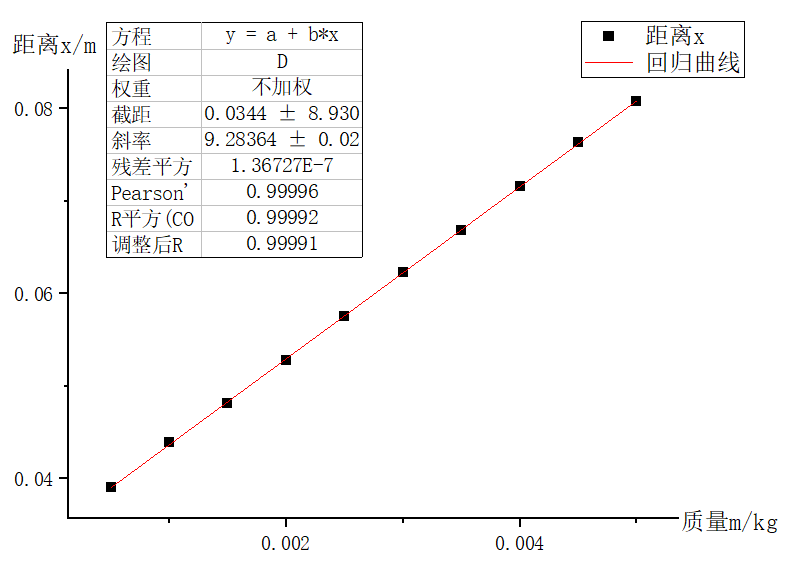
\includegraphics[width = 0.7\linewidth]{QQ图片20220401084307.png}
    \end{figure}
    由作图拟合结果也可计算得到
    \begin{equation*}
        k = \frac{g}{b} = 1.05 \mathrm{N}/\mathrm{m}
    \end{equation*}
    \item 用金属圈测量自来水的表面张力系数
    \begin{equation*}
        \overline{d} = \frac{\sum_{i=1}^3d_i}{3} = 0.0374\mathrm{m}
    \end{equation*}
    \[
        \sigma_d = \sqrt{\frac{\sum_{i = 1}^3\left(d_i-\overline{d}\right)^2 }{3-1}} = 0.00110 \mathrm{m}
        \]
        \[
            U_{d 0.95}=\sqrt{\left(t_{0.95} \frac{\sigma_{d}}{\sqrt{n}}\right)^{2}+\left(k_{P} \frac{\Delta_{B}}{C}\right)^{2}} = 0.0028\mathrm{m}
        \]
        \begin{equation*}
            \overline{l} = \frac{\sum_{i=1}^5l_i}{5} = 0.0940\mathrm{m}
        \end{equation*}
        \[
            \sigma_l = \sqrt{\frac{\sum_{i = 1}^5\left(l_i-\overline{l}\right)^2 }{5-1}} = 0.000377\mathrm{m}
            \]
            \[
                U_{l 0.95}=\sqrt{\left(t_{0.95} \frac{\sigma_{l}}{\sqrt{n}}\right)^{2}+\left(k_{P} \frac{\Delta_{B}}{C}\right)^{2}} = 0.0007\mathrm{m}
            \]
            由表面张力公式可得:
            \begin{equation*}
                \sigma = \frac{F-mg}{2l} = \frac{k(\overline{l}-l_0)}{2\pi\overline{d}} = 0.0594 \mathrm{N} /\mathrm{m}
            \end{equation*}
            对上式取微分并化为不确定度形式可得:
            \begin{equation*}
                \left(\frac{U_{\sigma}}{\sigma}\right)^{2}=\left(\frac{U_{k}}{k}\right)^{2}+\left(\frac{U_{l}}{\overline{l}-l_{0}}\right)^{2}+\left(\frac{U_{d}}{\overline{d}}\right)^{2}
            \end{equation*}
            这里我们通过数据处理1.的线性拟合结果可计算k的不确定度为:$\frac{U_{k}}{k} = 0.0022$
            代入计算可得
            \begin{equation*}
                \frac{U_{\sigma}}{\sigma} = 0.0915
            \end{equation*}
            即$U_\sigma = 0.005 \mathrm{N}/\mathrm{m}$
            \[
                \sigma = (0.0594 \pm 0.005) \mathrm{N}/\mathrm{m},P=0.95\]
    \item 金属丝测量洗洁精水(体积比1/1000)的表面张力系数
    \begin{equation*}
        \overline{l} = \frac{\sum_{i=1}^5l_i}{5} = 0.0820\mathrm{m}
    \end{equation*}
    \begin{equation*}
        \overline{s} = \frac{\sum_{i=1}^3s_i}{3} = 0.0417\mathrm{m}
    \end{equation*}
    由表面张力公式可得:
            \begin{equation*}
                \sigma = \frac{F-mg}{2l} = \frac{k(\overline{l}-l_0)}{2\overline{s}} = 0.0252 \mathrm{N} /\mathrm{m}
            \end{equation*}
    \item 金属丝测量其他浓度洗洁精水的表面张力,并绘制表面张力与浓度曲线
    
    通过原始数据可得
    \begin{equation*}
        \overline{l_1} = 0.0820 \mathrm{m} \quad
        \overline{l_2} = 0.0824 \mathrm{m} \quad
        \overline{l_3} = 0.0844 \mathrm{m}
    \end{equation*}
    通过表面张力公式
    \begin{equation*}
        \sigma = \frac{F-mg}{2l} = \frac{k(\overline{l}-l_0)}{2\overline{s}}
    \end{equation*}
    分别可得:
    \begin{equation*}
        \sigma_1 = 0.0252 \mathrm{N} /\mathrm{m} \quad
        \sigma_2 = 0.0302 \mathrm{N} /\mathrm{m}    \quad
        \sigma_3 = 0.0554 \mathrm{N} /\mathrm{m}
    \end{equation*}
    浓度(体积比)分别为$\frac{1}{100}\quad\frac{1}{10000}\quad\frac{1}{1000000}$

    结合上述得到的水和体积比为$\frac{1}{1000}$的表面张力数据,在origin中拟合结果如图:
    \begin{figure}[H]
        \centering
        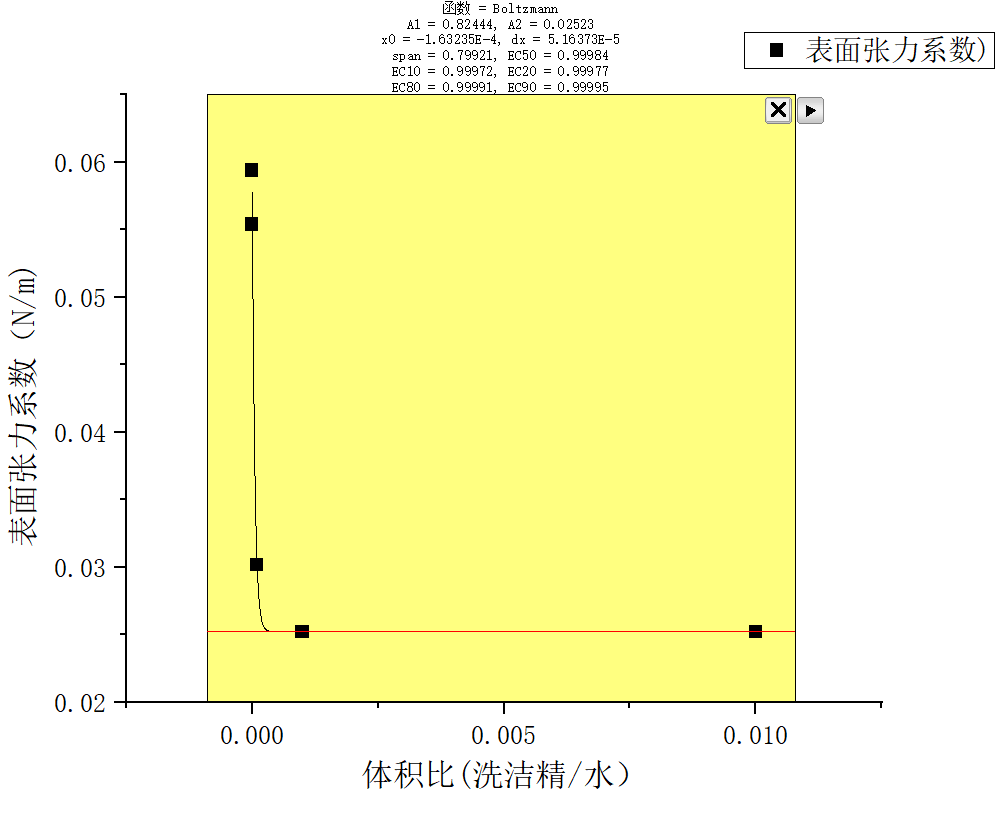
\includegraphics[width = 0.7\linewidth]{QQ截图20220401115904.png}
    \end{figure}
    \item 利用金属丝测量酒精表面张力系数
\end{enumerate}
\section{实验结果}
\begin{enumerate}
    \item 实验结果
\end{enumerate}
\section{思考题}
\begin{enumerate}
    \item 思考题
\end{enumerate}
\section{实验总结}
\begin{enumerate}
    \item 实验总结
\end{enumerate}
\end{document}